%!TEX root = mainfile.tex

\section{Photometry Exposure Times} % (fold)
\label{sec:exposure_times}
(Rahim, except~\ref{sub:full_width_at_half_maximum} Dorothy and Mike)

	The main aim of this project is to produce an observing strategy to view some of the earliest galaxies in the universe and map the epoch of reionization during which they were produced. An important aspect of this is therefore the viewing of the galaxies themselves and the time it will take to do so. The time required to view these galaxies depends not only on the telescope being used, but also the devices used. A charged coupled device (CCD) will be used to measure the light from these sources and so to calculate the times required to view these galaxies, these must be understood in more detail. The telescope or telescopes used during the observation of these galaxies will have different properties which will affect the time required to view the source. Some of these are discussed below.

	\subsection{Telescope Properties} % (fold)
	\label{sub:telescope_properties}
		\subsubsection{Mirror Reflectivity} % (fold)
		\label{ssub:mirror_reflectivity}
			One such factor that will increase the time required to view a source is the reflectivity of the mirrors used on the telescope. The mirror reflectivity, given as a percentage, is the amount of light reflected by the mirror. Some of the light is absorbed by the miror producing heat as it is not 100\% efficient meaning not all photons striking the mirror reach the the next mirror or the CCD. The reflectivity differs depending on the material used on the surface of the mirrors. Various optical coatings are produced and used depending on the wavelengths being observed, for example, the James Webb Space Telescope uses a gold coating which is particularly useful in the infrared region and is also very durable due to the inert nature of gold. The reflectivity of this gold coated mirror is in the region of 98\%--99\%\cite{Quantum_Coatings_Incorporated}. Other coatings regularly used include aluminium, which has a reflectivity in the region of 80\%--90\% and is utilised in the UV and IR range, as well as silver, which has a reflectivity in the range of 95\%--99\% and is utilised in the visible and IR range.
		% subsubsection mirror_reflectivity (end)

		\subsubsection{Telescope Throughput} % (fold)
		\label{ssub:telescope_throughput}
			The definition of throughput is the ratio of the flux detected by a particular instrument in a given filter and the incoming flux measured over an area equal to the area of the telescope primary mirror\cite{WIRCam_Throughput}. The throughput is therefore the percentage of photons striking the primary mirror that reach the CCD and are recorded. This contributes to the time required to observe a source as not all the photons striking the primary mirror, originating from the source, will reach the CCD. As the number of photons reaching the CCD is fewer, a larger portion of time is required to obtain the sought after signal-to-noise ratio and so the overall observation lasts a longer period of time.
		% subsubsection telescope_throughput (end)

		\subsubsection{Filters} % (fold)
		\label{ssub:filters}
			An astronomical filter is used on telescopes to remove light of unwanted wavelengths above and below a certain bandpass where a bandpass is a range of wavelengths that can pass through the filter. The width of this bandpass is commonly known as the bandwidth and is often used in astronomical calculations. The filter used will contain the specific wavelength being observed within the bandpass and reduce flux from other parts of the spectrum. A narrower filter will therefore ensure less background flux is observed reducing the error on the number of photons arriving from the source.

			A filter is usually denoted with the central wavelength and width of the filter. For example, one particular filter used on the James Webb Space Telescope is named F160N, denoting a central wavelength of \SI{1.6}{\micro\metre} and a narrow bandwidth. The bandwidth can then be found as it will be specific to the filter.

			The filter used is dependent on the redshifted wavelength of light from the source being observed. The wavelength of the redshifted light will be matched to a filter with the closest central wavelength to this wavelength. The bandpass of the telescope is the range of wavelengths that can pass through the filter and be measured as flux and so matching the redshifted wavelength to a filter with a similar central wavelength will allow the most flux from the source to be measured.
		% subsubsection filters (end)

		\subsubsection{Field of View} % (fold)
		\label{ssub:field_of_view}
			The field of view is specific to each telescope and gives the area of sky that is subtended by the CCD. This therefore depends on the CCD and the angle of sky subtended by each pixel. From this, the total area of sky imaged on the CCD can be determined. This is an important factor to take into account during the final observing strategy as, although a particular telescope may be quicker in finding a source, a larger field of view will mean more galaxies can be viewed. This therefore means a compromise must be produced to develop the optimum observing strategy.
		% subsubsection field_of_view (end)
	% subsection telescope_properties (end)

	\subsection{Charged Coupled Devices} % (fold)
	\label{sub:charged_coupled_devices}
		A charged coupled device or CCD is currently the detector of choice in astronomy and is used to produce images using incoming photons. A CCD works over a broad range of wavelengths and generally has high quantum efficiency within this range. They can vary in size from \SI{1.3}{\milli\metre} to up to \SI{70}{\milli\metre} across the diagonal. A larger size means more photosites and usually better image quality however the price of a CCD unfortunately rises exponentially with size ranging from \$60 to \$4000. They are still regarded as the best detectors available to astronomers and so are widely used in astronomical observations.

		CCDs consist of an array of metal-oxide semiconductor (MOS) capacitors, known as photo-detector junctions or photosites, formed on a silicon substrate. One pixel in the CCD can contain between one and a few of these capacitors. Each photosite contains a charge isolated from other photosites by a voltage applied through conductive channels on the surface of the silicon\cite{Diffraction_Limited_Imaging_Saha}. The MOS capacitor is structured with a metal electrode applied on top of a silicon substrate usually separated by a thin layer of insulation. At the beginning of each exposure, the electrodes are positively charged repelling holes in the substrate forming a depletion region which is an electrostatic potential well. Photons entering the substrate free electrons via the photoelectric effect and these are then attracted to the positively charged electrode and so are collected in the depletion region. The holes generated are repelled away from the depletion region and are lost in the substrate. The electrons generated can then be collected in the pixel and are counted to reproduce the pattern of the incident light producing an image.

		The photosites on a CCD are arranged in columns and lines convenient for the readout procedure. The array contains a special row of photosites on the bottom line known as the serial register. Upon completion of the exposure, the electrons in the columns of the array are clocked down one line with the bottom line entering the serial register. The serial register is then clocked into a charge detection node moving one pixel at a time. The electrons move along the row towards the charge detection node and upon completion of clocking each row, the next row up will drop into the serial register and be clocked in an identical fashion\cite{Astronomical_Image_Processing}. During this readout procedure, a shutter must be applied to prevent light generating further electrons. The readout time of a CCD can vary from a fraction of a second to around ten seconds.

		The CCD does however have numerous errors known as noise, which contribute to the integration time required to view the distant galaxies being examined in this project and so must be taken into account. The conversion of light to pixel values in a CCD leads to an inevitable noise being introduced into the image. This noise is the unwanted variations in pixel values and causes the image produced to differ from the one being observed. The noise incurred will make it more difficult to distinguish the source being observed hence increasing the integration time. For an electrical measuring system such as a CCD, a signal to noise ratio characterises the quality of the measurement taken where the signal to noise ratio ($\frac{S}{N}$) is the ratio of signal from the source being observed and signal produced by background radiation and other sources of noise. The main sources of noise for a CCD are the Poisson error, dark current, sky background and read noise, which are all described below.


		\subsubsection{Poisson Error} % (fold)
		\label{ssub:poisson_error}
			The Poisson error ($\sigma_\text{Poisson}$) or photon counting error is due to variations in the incoming flux of a source. As the photons from the source arrive randomly, the actual number arriving at a certain time or in a small time interval may differ from the average and so the error is on the detection of these photons. The Poisson error can be calculated quite simply as the error is the square root of the number of counts. This is shown in equation~(\ref{eq:poisson_error_sqrt_Ft}) where $F$ is the incoming flux and t is the exposure time.
			\begin{align}
				\sigma_\text{Poisson} = \sqrt{Ft} \label{eq:poisson_error_sqrt_Ft}
			\end{align}
		% subsubsection poisson_error (end)

		\subsubsection{Dark Current} % (fold)
		\label{ssub:dark_current}
			Dark current ($\sigma_\text{Dark}$), also known as thermal current, is due to the random generation of electrons and holes within the substrate of the MOS capacitor. Atoms in the silicon substrate of the CCD used are thermally excited and thus electrons are freed. These are then counted along with the electrons freed by photons from the object being observed. This occurs even when the CCD is not exposed to light, hence there is a steady creation of electrons, and this is called the dark or thermal current. As this is caused by thermal excitation, it strongly depends on the temperature at which the device is operating. At any given temperature, the rate at which electrons are freed is constant, however for every rise in temperature of 6 degrees Celsius, the dark current produced approximately doubles\cite{Astronomical_Image_Processing}. This relationship is shown in Figure~\ref{fig:dark_current_vs_temp}\cite{Southern_Observatory_throughput}.
			\begin{figure}[htbp]
				\centering
				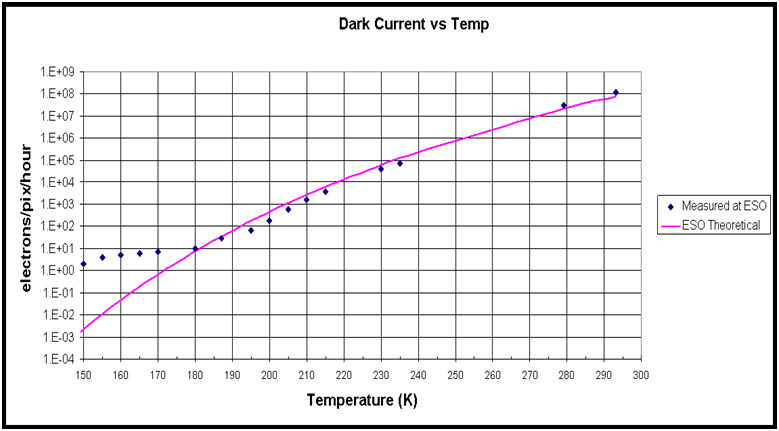
\includegraphics[width=0.6\textwidth]{../Images/Dark.png}
				\caption{A graph showing the relationship between dark current and temperature.\label{fig:dark_current_vs_temp}}
			\end{figure}

			Figure~\ref{fig:dark_current_vs_temp} shows that relationship between temperature and dark current for a custom designed CCD provided to the European Southern Observatory and shows clearly the increase in dark current at higher temperatures. CCD's are therefore cooled, often with the use of liquid nitrogen, to minimise this effect. The dark current itself is a relatively small electric current that flows through numerous photosensitive devices, and is one of the main sources of noise for a CCD. The dark noise contributed to the total noise can be calculated using the formula below where $D$ is the dark current in electrons per second per pixel, $t$ is the exposure time in seconds and N$_\text{pix}$ is the number of pixels in the CCD aperture.
			\begin{align}
				\sigma_\text{Dark} = \sqrt{DN_\text{pix}t}
			\end{align}
		% subsubsection dark_current (end)

		\subsubsection{Sky Background} % (fold)
		\label{ssub:sky_background}
			The sky background is the incoming light from the sky measured on the telescope that is not from the source being observed. The amount of sky background can vary at different wavelengths and is mainly due to light diffusion by the atmosphere. There are numerous sources that contribute towards the sky background such as airglow, zodiacal light and thermal radiation.

			Airglow is the atmospheric emission of photons at wavelengths from the near-UV to the near-IR range due to chemical reactions in the upper atmosphere\cite[p.~9]{An_atmospheric_radiation_model_for_Cerro_Paranal}. These chemical reactions lead to photon emissions due to the decay of electrons from an excited state in one of the reaction products. One such example is the emission in the near infrared region by OH radicals created from a reaction between ozone and hydrogen in the upper atmosphere\cite[p.~1]{MNRMNR11383}. Other processes contributing to airglow are the recombination of ions originally ionised by the sun, and the luminescence of cosmic rays striking the upper atmosphere. Airglow therefore produces a faint glow and can be seen in Figure~\ref{fig:air_glow_in_upper_atmosphere}.
			% \begin{figure}[htbp]
			% 	\centering
			% 	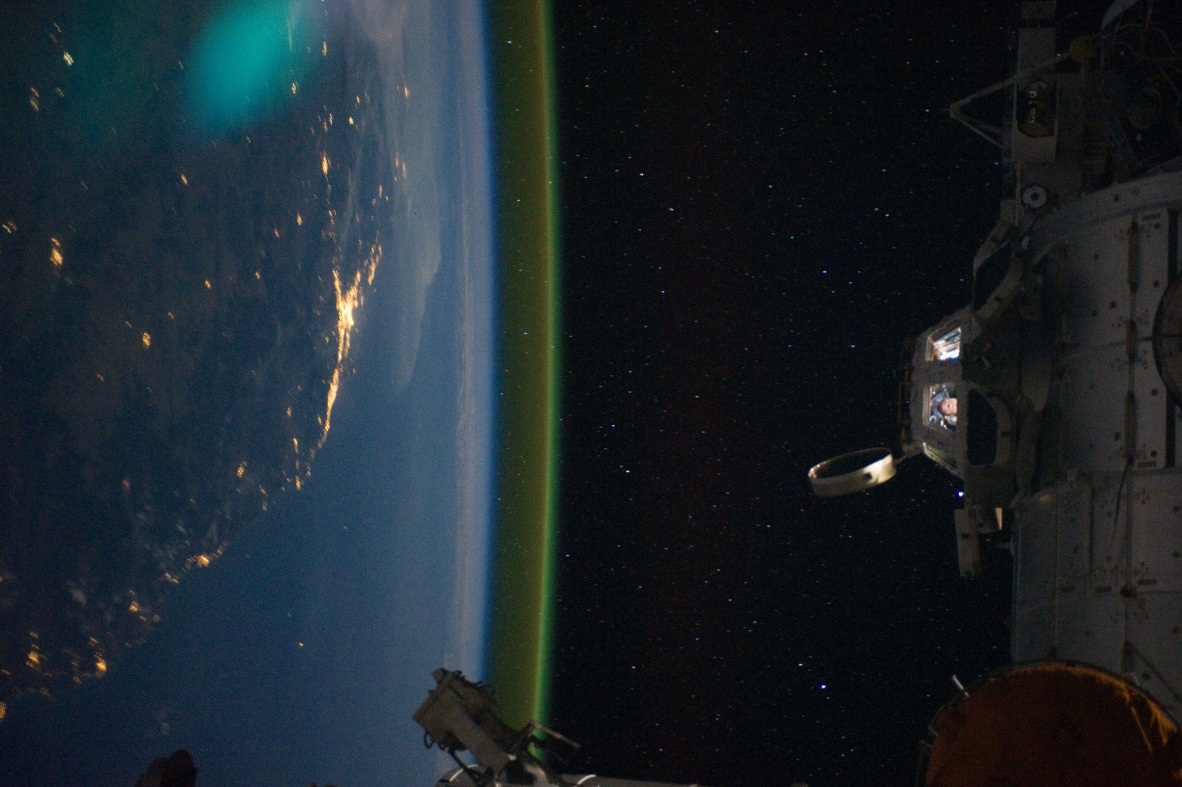
\includegraphics[width=0.7\textwidth]{../Images/airglow_in_upper_atmosphere.jpeg}
			% 	\caption{Airglow in the upper atmosphere as observed from the International Space Station\cite{ISS028_E_050185}}\label{fig:air_glow_in_upper_atmosphere}
			% \end{figure}
			% \begin{figure}[htbp]
			% 	\centering
			% 	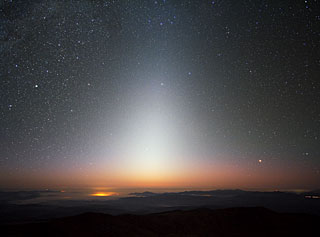
\includegraphics[width=0.7\textwidth]{../Images/zodiacal_light.jpeg}
			% 	\caption{An image of zodiacal light above the earth}\label{fig:air_glow_in_upper_atmosphere}
			% \end{figure}
			\begin{figure}[htbp]
				\begin{minipage}[c]{0.5\linewidth}
					\centering
					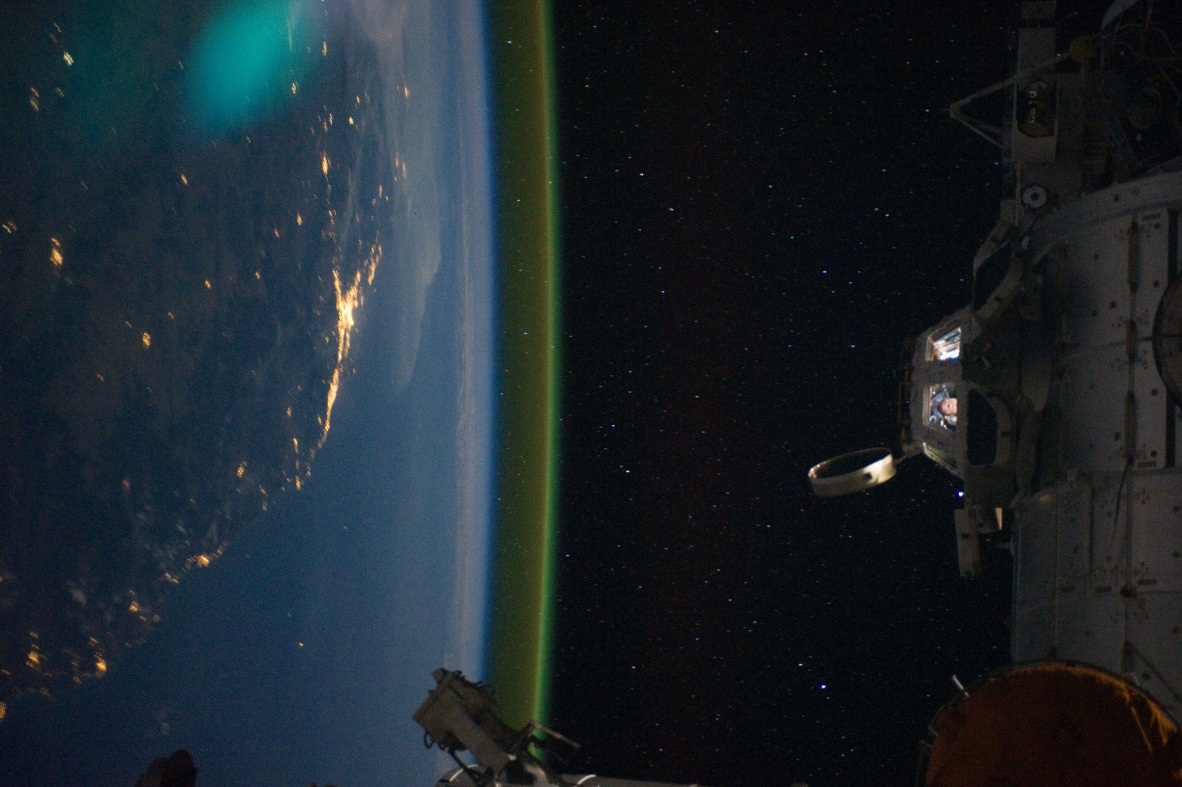
\includegraphics[height=4.5cm]{../Images/airglow_in_upper_atmosphere.jpeg}
				\end{minipage}
				\begin{minipage}[c]{0.5\linewidth}
					\centering
					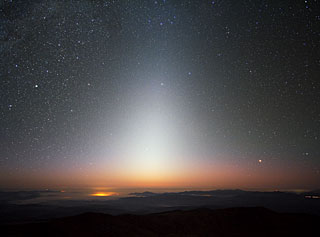
\includegraphics[height=4.5cm]{../Images/zodiacal_light.jpeg}
				\end{minipage}
				\caption{Left: Airglow in the upper atmosphere as observed from the International Space Station\cite{ISS028_E_050185}. Right: An image of zodiacal light above the earth}\label{fig:air_glow_in_upper_atmosphere}
			\end{figure}

			Another of the contributors to the sky background is zodiacal light which is the scattering of sunlight off interplanetary dust\cite[p.~5--6]{MNRMNR21602}. This can be seen in Figure~\ref{fig:air_glow_in_upper_atmosphere} below. This causes a faint white glow that can be best seen before sunrise or after sunset but is generally so faint it cannot be seen over moonlight or light pollution. The dust in the solar system forms a thick lens shape cloud known as the interplanetary dust cloud or zodiacal cloud and it is off this cloud that light from the Sun is scattered. Zodiacal light is mainly seen in the ecliptic plane, the plane of the solar system, as most of the dust making up this cloud is located in this plane. Another similar effect to this is the gegenschein, or counter shine, which is a faint glow in the antisolar direction\cite{Observational_Studies_of_Interplanetary_Dust}. At this point, the zodiacal light is enhanced by backscattering off interplanetary dust producing a small brightening in this part of the sky.

			Background from zodiacal light can however be greatly reduced by observing outside of the ecliptic plane as this is where the flux of photons due to zodiacal light is weakest. This can be seen in Figure~\ref{fig:air_glow_in_upper_atmosphere_graph} below which shows the flux of photons as a function of angle to the ecliptic plane.
			\begin{figure}[htbp]
				\centering
				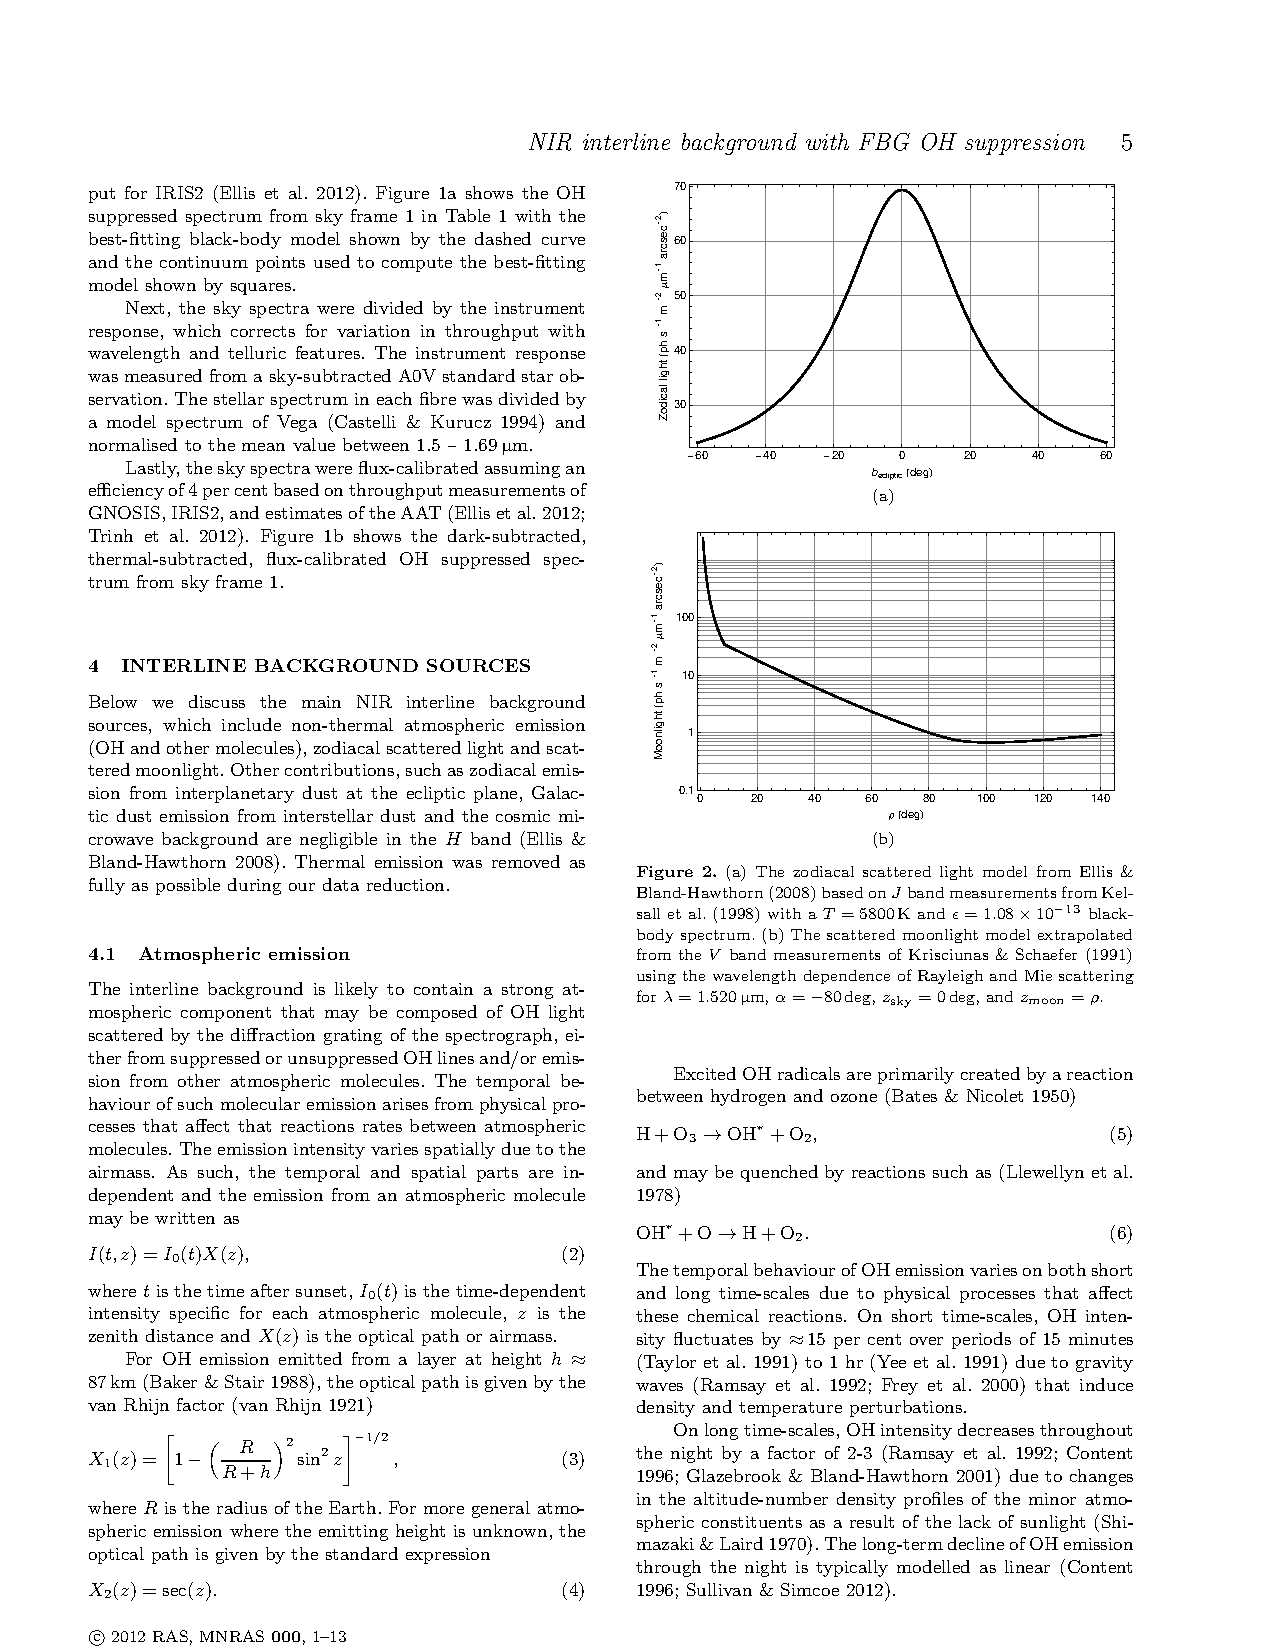
\includegraphics[trim = 110mm 198mm 25mm 30mm, clip, width=0.4\textwidth]{../Images/zodiacal_Light_graph.pdf}
				\caption[Zodiacal light vs angle]{The relationship between intensity of zodiacal light and the angle to the plane of the solar sytem}\label{fig:air_glow_in_upper_atmosphere_graph}
			\end{figure}

			The zodiacal light is strongest at a very small angle to the ecliptic plane but significantly decreases as the angle increases and so viewing well outside the ecliptic plane should considerably reduce background from zodiacal light\cite{Zodiacal_Light_over_La_Silla}.Thermal radiation in the atmosphere by greenhouse gases also contributes to the sky background and is due to the absorption and emission of radiation from the Sun into the atmosphere in the mid-IR region. In this case, observations in the mid- and far-IR region must be carried out from outside the atmosphere\cite{Extragalactic_Astronomy_and_Cosmology}. The sky background is therefore primarily an issue for ground based telescopes as they can incur a large background number of photons compared to the number of photons arriving from the source being observed.

			As space based telescopes are situated outside of the atmosphere, they avoid almost all of this background with their main source of background coming in the form of zodiacal light or thermal background due to radiation from the Sun. This can be calculated by first determining the number of photons from this thermal background before converting to a noise represented by the number of electrons excited in the CCD. The number of photons, $N\gamma$, can be calculated using the formula,
			\begin{align}
				N_\gamma &= \frac{2k^3 T^3 \epsilon}{h^3 c^2} {\left[ \e{-x}\left( x^2 + 2x + 2 \right) \right]}^{x_2}_{x_1},
			\end{align}
			where $x=\frac{h\nu}{kt}$, $\nu$ is frequency, $k$ is the Boltzmann constant, $t$ is temperature, $h$ is Planck's constant, $c$ is the speed of light and $\epsilon$ is the emissivity. $x_1$ is the bluer end of the filter, i.e.\ the shorter wavelength whilst $x_2$ is the redder end of the filter, i.e.\ the longer wavelength. The full derivation of this can be seen in appendix~\ref{app:derivation_of_thermal_background}. This can then be used to calculate the number of electrons per second per pixel ($N_e$) on the CCD contributing towards the background via the formula,
			\begin{align}
				N_e &= N_\gamma A\epsilon_{\text{th}}\Omega_{\text{pix}},
			\end{align}
			Where $A$ is the collecting area of the telescope, $\epsilon_{\text{th}}$ is the throughput of the filter used and $\Omega_{\text{pix}}$ is the solid angle subtended by each pixel in steradians. Completing this calculation for the Hubble Space telescope gives a value of $N_e$ of \SI{0.02}{\electron\per\second\per\pixel}. Whilst this is not the dominant source of background for the Hubble telescope, this may be used to calculate a rough estimate of the thermal background of other space based telescopes such as Euclid and JWST which are located at the second Lagrange point, well away from any atmospheric background.

			The total sky background is measured to be $B$ photons per second per pixel and the noise contributed can be calculated using the formula below where $t$ is the exposure time and $N_\text{pix}$ is the number of pixels in the CCD aperture.
			\begin{align}
				\sigma_\text{Sky} = \sqrt{BN_\text{pix}t}
			\end{align}
		% subsubsection sky_background (end)

		\subsubsection{Read Noise} % (fold)
		\label{ssub:read_noise}
			When the electrons accumulated by the CCD are being read or clocked off and converted to a voltage, a readout noise ($\sigma_\text{RN}$), a small, random variation generated by the CCD's charge detection node is added. This noise is expressed as a number of electrons per second per pixel and is a fundamental trait of CCD's. It will, unfortunately, occur in all CCD's, from ones used in simple webcams to those used on the Hubble Space Telescope\cite{Understanding_CCD_Read_Noise}. The read noise contributed to the total noise can be calculated using the formula below where $R$ is the read noise of the CCD in electrons and $N_\text{pix}$ is the number of pixels in the CCD aperture.
			\begin{align}
				\sigma_\text{RN} = R\sqrt{N_\text{pix}}
			\end{align}
		% subsubsection read_noise (end)
	% subsection charged_coupled_devices (end)

	\subsection{Signal-to-Noise Ratio} % (fold)
	\label{ssub:signal_to_noise_ratio}
		The quality of a CCD image is quantified by a signal-to-noise ratio which can be established from the source signal and all noise contributions. The different types of noise discussed above, all contribute to a total noise ($\sigma$) in the received signal which can be calculated using equation~(\ref{eq:total_noise_in_recieved_signal}).
		\begin{align}
			\sigma^{2} = \sigma_{Poisson}^{2} + \sigma_{Dark}^{2} + \sigma_{Sky}^{2} + \sigma_{RN}^{2} \label{eq:total_noise_in_recieved_signal}
		\end{align}
		As the CCD is exposed to incoming light, both the background and the source signal build up. The background is randomly and evenly distributed and so also contributes to the peak of the signal which therefore sits as a peak or peaks above a layer of background and so can be distinguished. This can be seen on Figure~\ref{fig:signal_noise_accumulation} below where B is labelled in the region of background\cite{Signal_to_Noise_Ratio}.
		\begin{figure}[htbp]
			\centering
			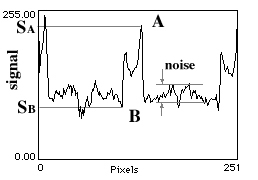
\includegraphics[width=0.4\textwidth]{../Images/SNR.png}
			\caption{The accumulation of signal, background and noise.\label{fig:signal_noise_accumulation}}
		\end{figure}

		The signal-to-noise ratio is therefore the total number of photons from the source reaching the CCD divided by the total noise for a given exposure time. As the exposure time increases, both signals, from source and background, cause an increase in counts establishing the signal more clearly. The signal-to-noise ratio is therefore also dependant on the exposure time although it is common for astronomers to decide on a signal-to-noise ratio to be obtained before calculating an exposure time.
		\begin{align}
			\frac{S}{N} = \frac{Ft}{\sigma} =\frac{Ft}{\sqrt{\sigma_\text{Poisson}^{2} + \sigma_\text{Dark}^{2} + \sigma_\text{Sky}^{2} + \sigma_{RN}^{2}}}
		\end{align}
		Either the signal-to-noise ratio or exposure time can then be calculated using the equation shown below commonly known as the CCD equation.
		\begin{align}
			\frac{S}{N} = \frac{Ft}{\sqrt{(F + BN_\text{pix} + DN_\text{pix})t + R{^2}N_\text{pix}}}
		\end{align}
		$F$ is the incident number of photons from the source per second, $t$ is the exposure time, $D$ is the dark current in electrons per second per pixel, $B$ is the sky background in photons per second per pixel and $R$ is the read noise in electrons. $N_\text{pix}$ is the number of pixels within the aperture area of the CCD and so is the number of pixels that are clocked to produce an image. This is dependent on the either the angular resolution of the telescope or the angular size of the object being observed depending on which is the limiting factor of the telescope and for photometry, can be calculated using equation~(\ref{eq:number_of_pixels_limiting}) below. The limiting factor becomes the FWHM in the equation and is discussed in Sections~\ref{sub:astronomical_seeing} and~\ref{sub:full_width_at_half_maximum} whilst $\theta_\text{pixel}$ is the angle subtended on the sky by one pixel. Observations on the James Webb Space Telescope will produce images with a signal-to-noise ratio of 10 indicating the current image quality desired.
		\begin{align}
			N_\text{pix} = \pi \left(\frac{4 \times \text{FWHM}}{\theta_\text{pixel}}\right)^2 \label{eq:number_of_pixels_limiting}
		\end{align}
	% subsubsection signal_to_noise_ratio (end)
% section exposure_times (end)
